\section{Réponse fréquentielle des SLCI}

\marginnote{\xpComp{SLCI}{11}}

\subsection{Définitions}

\marginnote{
\begin{itemize}
\item $T=\dfrac{2\pi}{\omega}$ : la période de la sinusoïde en $\text{s}$;
\item $f=\dfrac{1}{T}$ : fréquence de la sinusoïde en $\text{Hz}$.
\item $A$ : l'amplitude de la sinusoïde;
\item $\omega$ : la pulsation en $\text{rad/s}$;
\item $\varphi$ : la phase à l'origine en $\text{rad}$.
\end{itemize}}


On peut définir un signal sinusoïdal sous la forme $
f(t)=A \sin(\omega \cdot t + \varphi)
$ et on note :


Une étude harmonique consiste en solliciter le système par des sinusoïdes de pulsations différentes et d'observer son comportement en régime permanent. Le diagramme de Bode est constitué d'un diagramme de gain (rapport des amplitudes des sinus en régime permanent) et d'un diagramme de phase (déphasage des sinus en régime permanent). 


\begin{defi}[Gain \& Phase]
Soit $H(p)$ une fonction de transfert. On pose $p=j\omega$ et on note :  
\begin{itemize}
\item $H_{\text{dB}}\left( \omega\right) =20\log |H(j\omega)|$ le gain décibel de la fonction de transfert;
\item $\varphi\left( \omega\right) = \text{Arg}\left(H(j\omega) \right)$.
\end{itemize}
\end{defi}

\begin{resultat}
On note $H(p)=G_1(p)G_2(p)$. On a :
\begin{itemize}
\item $H_{\text{dB}}\left( \omega\right) =G1_{\text{dB}}\left( \omega\right)+G2_{\text{dB}}\left( \omega\right)$;
\item $\varphi\left( \omega\right)  =\text{Arg}\left(G1_{\text{dB}}\left( \omega\right)\right)+\text{Arg}\left(G2_{\text{dB}}\left( \omega\right)\right)$.
\end{itemize}
\end{resultat}
%\begin{tikzpicture}[xscale=7/4]
%\begin{scope}[yscale=3/40]
%\semilog{-2}{2}{-20}{20}
%\BodeAmp[cyan,thin,samples=100]{-2:2}
%{\POAmpAsymp{6}{0.3}}
%\BodeAmp[cyan,thick]{-2:2}{\POAmp{6}{0.3}}
%\end{scope}
%\begin{scope}[yshift=-2.5cm,yscale=3/90]
%\semilog{-2}{2}{-90}{0}
%\BodeArg[cyan,samples=100,thin]{-2:2}{\POArgAsymp{6}{0.3}}
%\BodeArg[cyan,thick]{-2:2}{\POArg{6}{0.3}}
%\end{scope}
%\end{tikzpicture}
\vspace{-.8cm}

\subsection{Gain}

\begin{marginfigure}[-.5cm]
\centering
\begin{tikzpicture}[xscale=7/7]
\tikzset{
semilog lines/.style={thin, bleuxp}, 
semilog lines 2/.style={semilog lines,bleuxpc},
semilog half lines/.style={semilog lines 2,dotted },
semilog label x/.style={semilog lines,below,font=\tiny,black},
semilog label y/.style={semilog lines,right,font=\tiny,black}
}
\begin{scope}[yscale=3/50]
\semilog{-2}{2}{0}{20}
\BodeAmp[ultra thick,orangexp]{-2:2}{\KAmp{2}}

\draw (0,8) node [above] {\footnotesize $20 \log K$};
\end{scope}
\begin{scope}[yshift=-1.2cm,yscale=1/50]
\UniteDegre
\OrdBode{30}
\semilog{-2}{2}{-30}{30}
\draw [ultra thick,orangexp] (-2,0) -- (2,0) node [above,midway,black]{\footnotesize 0\degre};
\end{scope}
\end{tikzpicture}
\end{marginfigure}



\begin{resultat}[Diagramme de Bode d'un gain pur]
\begin{itemize}
\item Fonction de transfert : $H(p)=K$.
\item Diagramme de gain : droite horizontale d'ordonnée $20 \log K$.
\item Diagramme de phase: droite horizontale d'ordonnée~0\degre.
\end{itemize}
\end{resultat}

\subsection{Intégrateur}


\begin{resultat}[Diagramme de Bode d'un intégrateur]
\begin{itemize}
\item Fonction de transfert : $H(p)=\dfrac{K}{p}$.
\item Diagramme de gain asymptotique : droite de pente $-{20}\text{dB/decade}$ passant par le point $(1,20\log K)$.
\item Diagramme de phase asymptotique : droite horizontale d'ordonnée $-90$ \degre.
\end{itemize}
\end{resultat}

\begin{marginfigure}[-4cm]
\begin{tikzpicture}[xscale=7/7]
\tikzset{
semilog lines/.style={thin, bleuxp}, 
semilog lines 2/.style={semilog lines,bleuxpc},
semilog half lines/.style={semilog lines 2,dotted },
semilog label x/.style={semilog lines,below,font=\tiny,black},
semilog label y/.style={semilog lines,right,font=\tiny,black}
}
\begin{scope}[yscale=3/300]
\OrdBode{40}
\semilog{-2}{2}{-20}{60}
\BodeAmp[orangexp,ultra thick]{-2:2}{\IntAmp{10}}
%\draw (-1,28) node {\footnotesize $20\log K$, 0 dB/d\'ecade};
\draw (0,20) node [above right] {\footnotesize $(1,20\log K)$};
\draw (0,20) node {\huge $\cdot$};
%\draw (.7,0)  node {\Huge $\cdot$} node [above right]{\footnotesize $\dfrac{1}{\tau}$};
\end{scope}
\begin{scope}[yshift=-1.2cm,yscale=1/70]
\UniteDegre
\OrdBode{45}
\semilog{-2}{2}{-90}{0}
\BodeArg[orangexp,ultra thick]{-2:2}{\IntArg{10}}
\end{scope}
\end{tikzpicture}
\end{marginfigure}



\subsection{Dérivateur}

\begin{marginfigure}
\begin{tikzpicture}[xscale=7/7]
\tikzset{
semilog lines/.style={thin, bleuxp}, 
semilog lines 2/.style={semilog lines,bleuxpc},
semilog half lines/.style={semilog lines 2,dotted },
semilog label x/.style={semilog lines,below,font=\tiny,black},
semilog label y/.style={semilog lines,right,font=\tiny,black}
}
\begin{scope}[yscale=3/300]
\OrdBode{30}
\semilog{-2}{2}{-30}{90}

\BodeAmp[orangexp,ultra thick]{-2:2}{\KAmp{10}-\IntAmp{1}}
%\draw (-1,28) node {\footnotesize $20\log K$, 0 dB/d\'ecade};
\draw (0,20) node [above left] {\footnotesize $(1,20\log K)$};
\draw (0,20) node {\huge $\cdot$};
%\draw (.7,0)  node {\Huge $\cdot$} node [above right]{\footnotesize $\dfrac{1}{\tau}$};
\end{scope}
\begin{scope}[yshift=-1.9cm,yscale=1/70]
\UniteDegre
\OrdBode{30}
\semilog{-2}{2}{0}{90}
\BodeArg[orangexp,ultra thick]{-2:2}{-\IntArg{10}}
\end{scope}
\end{tikzpicture}
\end{marginfigure}

\begin{resultat}[Diagramme de Bode d'un dérivateur]
\begin{itemize}
\item Fonction de transfert : $H(p)={K}{p}$.
\item Diagramme de gain asymptotique : droite de pente ${20}\text{dB/decade}$ passant par le point $(1,20\log K)$.
\item Diagramme de phase asymptotique : droite horizontale d'ordonnée $+90$ \degre.
\end{itemize}
\end{resultat}


\subsection{Systèmes d'ordre 1}


\begin{marginfigure}
\begin{tikzpicture}[xscale=7/7]
\tikzset{
semilog lines/.style={thin, bleuxp}, 
semilog lines 2/.style={semilog lines,bleuxpc},
semilog half lines/.style={semilog lines 2,dotted },
semilog label x/.style={semilog lines,below,font=\tiny,black},
semilog label y/.style={semilog lines,right,font=\tiny,black}
}
\begin{scope}[yscale=3/50]
\semilog{-2}{2}{0}{30}

\BodeAmp[orangexp,thin,samples=100]{-2:2}{\POAmpAsymp{20}{0.2}}
\BodeAmp[orangexp,ultra thick]{-2:2}{\POAmp{20}{0.2}}
\draw (-1,28) node {\footnotesize $20\log K$, 0 dB/d\'ecade};
\draw (1.7,20) node {\footnotesize $-$20 dB/d\'ecade};
\draw [dashed,thick,bleuxp] (.7,0) -- (.7,25);
\draw (.7,0)  node {\Huge $\cdot$} node [above right]{\footnotesize $\dfrac{1}{\tau}$};
\end{scope}
\begin{scope}[yshift=-0.5cm,yscale=1/50]
\UniteDegre
\OrdBode{30}
\semilog{-2}{2}{-90}{0}
\BodeArg[orangexp,samples=100,thin]{-2:2}{\POArgAsymp{20}{0.2}}
\BodeArg[orangexp,ultra thick]{-2:2}{\POArg{20}{0.2}}
\end{scope}
\end{tikzpicture}
\end{marginfigure}

\begin{resultat}[Diagramme de Bode d'un système du premier ordre]
\begin{itemize}
\item Fonction de transfert : $H(p)=\dfrac{K}{1+\tau p}$.
\item Diagramme de gain asymptotique : 
\begin{itemize}
\item pour $\omega<\dfrac{1}{\tau}$ : droite horizontale d'ordonnée $20 \log K$;
\item pour $\omega>\dfrac{1}{\tau}$ : droite de pente $-{20}\text{dB/decade}$.
\end{itemize}
\item Diagramme de phase asymptotique : 
\begin{itemize}
\item pour $\omega<\dfrac{1}{\tau}$ : droite horizontale d'ordonnée 0 \degre;
\item pour $\omega>\dfrac{1}{\tau}$ : droite horizontale d'ordonnée $-90$ \degre.
\end{itemize}
\end{itemize}
\end{resultat}



\subsection{Systèmes d'ordre 2}


\begin{resultat}[Diagramme de Bode d'un système du deuxième ordre]
\begin{itemize}
\item Fonction de transfert : $H(p)=\dfrac{K}{1+\dfrac{2\xi}{\omega_0}+\dfrac{p^2}{\omega_0^2}}$.
\end{itemize}
\begin{center}
\textbf{Cas où $\xi<1$.}
\end{center}
\begin{itemize}
\item Diagramme de gain asymptotique : 
\begin{itemize}
\item pour $\omega<\omega_0$ : droite horizontale d'ordonnée $20 \log K$;
\item pour $\omega>\omega_0$ : droite de pente $-{40}\text{dB/decade}$.
\end{itemize}
\item Diagramme de phase asymptotique : 
\begin{itemize}
\item pour $\omega<\omega_0$ : droite horizontale d'ordonnée 0 \degre;
\item pour $\omega>\omega_0$ : droite horizontale d'ordonnée $-180^{\text{o}}$.
\end{itemize}
\end{itemize}


Dans le \textbf{cas où $\xi>1$}, le dénominateur admet deux racines (à partie réelle négative) et peut se mettre sous la forme  $\left(1+\tau_1 p \right)\left(1+\tau_2 p \right)$. On se ramène alors au tracé du produit de deux premier ordre.
\end{resultat}

\begin{marginfigure}[-6cm]
\begin{tikzpicture}[xscale=7/7]
\tikzset{
semilog lines/.style={thin, bleuxp}, 
semilog lines 2/.style={semilog lines,bleuxpc},
semilog half lines/.style={semilog lines 2,dotted },
semilog label x/.style={semilog lines,below,font=\tiny,black},
semilog label y/.style={semilog lines,right,font=\tiny,black}
}
\begin{scope}[yscale=3/150]
\OrdBode{20}
\semilog{-2}{2}{-60}{40}
\BodeAmp[orangexp,thin,samples=150]{-2:2}{\SOAmpAsymp{10}{0.2}{.9}}
\BodeAmp[orangexp,ultra thick,samples=150]{-2:2}{\SOAmp{10}{0.2}{.9}}
\draw (-1.5,28) node {\footnotesize $20\log K$};
\draw (1.1,10) node {\footnotesize $-$40 dB/d\'ecade};
\draw [dashed,ultra thick,bleuxp] (-.08,-60) -- (-.08,25);
\draw (-.08,-60)  node {\Huge $\cdot$} node [above right]{\footnotesize $\omega_0$};
\end{scope}
\begin{scope}[yshift=-1.7cm,yscale=1/90]
\UniteDegre
\OrdBode{45}
\semilog{-2}{2}{-180}{0}
\BodeArg[orangexp,samples=100,thin]{-2:2}{\SOArg{10}{0.2}{.9}}
\BodeArg[orangexp,ultra thick]{-2:2}{\SOArg{10}{0.2}{.9}}
\end{scope}
\end{tikzpicture}
\end{marginfigure}


\marginnote{En utilisant la figure précédente, on lit un gain maximal de \SI{30}{dB} soit $\indice{A}{max}=10^{1,5}$ et on a un gain de $K=10$. $\xi$ est solution de $10^{1,5} \times 2\xi\sqrt{1-\xi^2} - 10 = 0$.}
\begin{resultat}[Phénomène de résonance]

Le phénomène de résonance s'observe lorsque $\xi<\dfrac{\sqrt{2}}{2}$. La pulsation de résonance est inférieure à la pulsation propre du système :
$\omega_r = \omega_0\sqrt{1-2\xi^2}$.

\`A la résonance, l'amplitude maximale est de 
$A_{\text{max}} = \dfrac{K}{2\xi\sqrt{1-\xi^2}}.$
(Attention, sur le diagramme de Bode, on lit $20\log A_{\text{max}}$ lorsque $\omega=\omega_r$.)
\end{resultat}

\clearpage

\subsection{Retard}

\begin{marginfigure}
\begin{tikzpicture}[xscale=7/7]
\tikzset{
semilog lines/.style={thin, bleuxp}, 
semilog lines 2/.style={semilog lines,bleuxpc},
semilog half lines/.style={semilog lines 2,dotted },
semilog label x/.style={semilog lines,below,font=\tiny,black},
semilog label y/.style={semilog lines,right,font=\tiny,black}
}
\begin{scope}[yscale=4/50]
\UnitedB
\OrdBode{5}
\semilog{0}{3}{-10}{10}
\BodeAmp[orangexp,ultra thick]{0:3}{\RetAmp{.08}}
\end{scope}
\begin{scope}[yshift=-1.5cm,yscale=4/180]
\UniteDegre
\OrdBode{30}
\semilog{0}{3}{-90}{0}
%\BodeArg[samples=100]{0:3}{\RetArg{0.08}}%\RetArg{0.08}}
\BodeArg[orangexp,ultra thick]{0:3}{\RetArg{0.08}}
\end{scope}
\end{tikzpicture}
\end{marginfigure}

\begin{resultat}[Diagramme de Bode d'un retard pur]
\begin{itemize}
\item Fonction de transfert : $H(p)=e^{-Tp}$.
\item Diagramme de gain asymptotique : gain nul.
\item Diagramme de phase asymptotique : $\text{arg}\left( H(p) \right)=-\tau\omega$.
\end{itemize}
\end{resultat}


\subsection{Tracé du diagramme de Bode}

\begin{methode}[1 : Sommation dans le diagramme de Bode]
\begin{enumerate}
\item Décomposer la fonction de transfert à tracer en fonction de transfert élémentaire (fonctions de transfert élémentaires vues ci-dessus).
\item Tracer chacune des fonctions de transfert.
\item Sommer les tracés dans le diagramme de gain et dans le diagramme des phases.
\end{enumerate}
\end{methode}

\begin{methode}[2 : Tableau de variations]
\begin{enumerate}
\item Décomposer la fonction de transfert à tracer en fonction de transfert élémentaire (fonctions de transfert élémentaires vues ci-dessus).
\item Réaliser un tableau de variation : pour chacune des fonctions élémentaires, donner les pulsations de coupure et les pentes.
\item Sommer les pentes.
\item Déterminer le gain en basse fréquence si la classe est nulle ou déterminer le gain pour une pulsation donnée si la classe est non nulle.
\item Tracer le diagramme de Bode.
\end{enumerate}
\end{methode}

Application : tracer de $F(p)=\dfrac{10}{p\left(1+0,9p\right)}$.

\begin{center}
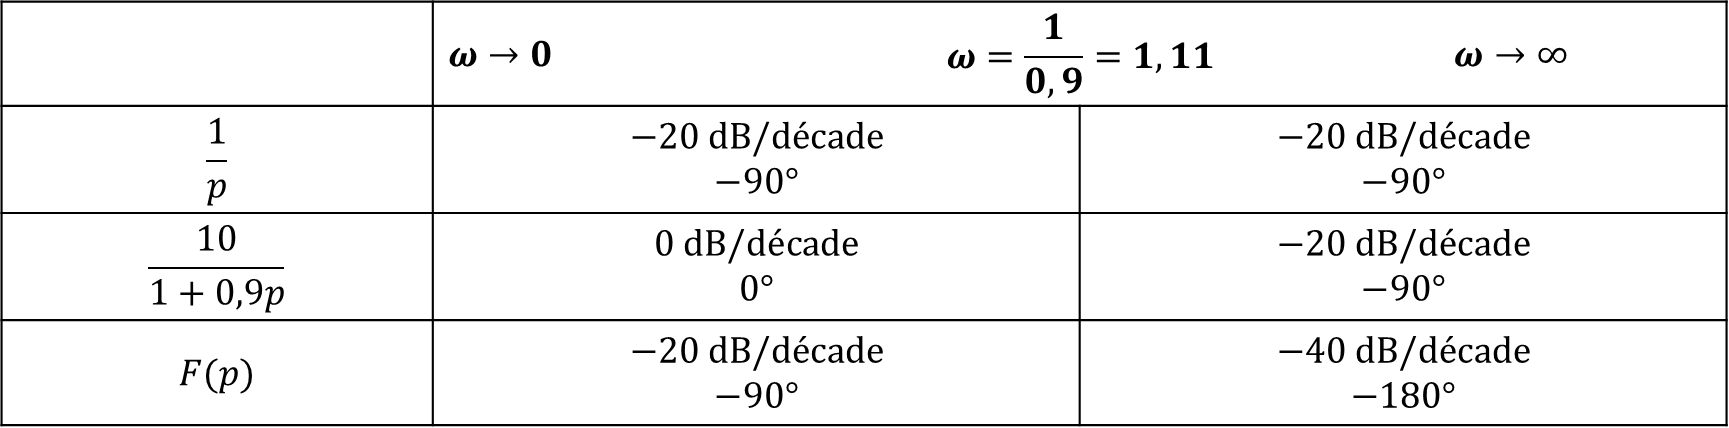
\includegraphics[width=.85\linewidth]{variations}
\end{center}

Ici le système est de classe 1. Pour $\omega << 1,11$, $F(p)\simeq \dfrac{10}{p}$. Pour $\omega = 0,01$, on a donc $\indice{G}{dB}(0,01) \simeq 20\log 10 - 20\log (0,1) = 20-20\times (-2) = 60$.

\begin{figure}[!h]
\centering
\begin{tikzpicture}[xscale=14/7]
\tikzset{
semilog lines/.style={thin, bleuxp}, 
semilog lines 2/.style={semilog lines,bleuxpc},
semilog half lines/.style={semilog lines 2,dotted },
semilog label x/.style={semilog lines,below,font=\tiny,black},
semilog label y/.style={semilog lines,right,font=\tiny,black}
}
\begin{scope}[yscale=3/150]
\OrdBode{20}
\semilog{-2}{2}{-60}{60}
\BodeAmp[bleuxp,thick,samples=150]{-2:2}{\POAmpAsymp{10}{.9}+\IntAmp{1}}
\BodeAmp[orangexp,ultra thick,samples=150]{-2:2}{\POAmp{10}{.9}+\IntAmp{1}}
\end{scope}
\begin{scope}[yshift=-1.7cm,yscale=1/90]
\UniteDegre
\OrdBode{45}
\semilog{-2}{2}{-180}{0}
\BodeArg[bleuxp,samples=100,thick]{-2:2}{\POArgAsymp{10}{.9}+\IntArg{1}}
\BodeArg[orangexp,ultra thick]{-2:2}{\POArg{10}{.9}+\IntArg{1}}
\end{scope}
\end{tikzpicture}
\end{figure}
